\documentclass[letterpaper, 10 pt, conference]{ieeeconf}
\usepackage{graphicx}

\overrideIEEEmargins

\usepackage[utf8]{inputenc}
\usepackage[T1]{fontenc}
\usepackage{graphics}
\usepackage{amsmath}
\usepackage{amssymb}
\usepackage{booktabs}

\title{\LARGE \bf
Clasificaci\'on multi-clase de art\'iculos de la BBC mediante fine-tuning de BERT
}

\author{Juan Manuel Gómez Cárdenas, Andrés Javier Rambal Vecino, Ricardo Andrés Pabón Masapanta}

\begin{document}

\maketitle
\thispagestyle{empty}
\pagestyle{empty}

%%%%%%%%%%%%%%%%%%%%%%%%%%%%%%%%%%%%%%%%%%%%%%%%%%%%%%%%%%%%%%%%%%%%%%%%%%%%%%%%
\section{Introducci\'on}

La clasificaci\'on autom\'atica de noticias es una tarea cl\'asica de Procesamiento del Lenguaje Natural (PLN) con aplicaciones en organizaci\'on editorial y recomendaci\'on de contenidos. Los modelos recurrentes dominaron esta tarea durante a\~nos, pero su naturaleza secuencial limita la captura de dependencias largas \cite{rnn_vs_tx}. La introducci\'on de la auto-atenci\'on en el \emph{Transformer} \cite{attention} cambi\'o el panorama al permitir el procesamiento paralelo de secuencias y modelar relaciones de largo alcance. Sobre esa arquitectura, BERT \cite{bert} introdujo un preentrenamiento bidireccional con \emph{Masked Language Modeling} cuyas representaciones contextuales transfieren bien a tareas \emph{downstream} mediante \emph{fine-tuning}.

En este trabajo abordamos la clasificaci\'on de art\'iculos del dataset \emph{BBC News} \cite{bbcdata} en cinco categor\'ias tem\'aticas (\emph{business, entertainment, politics, sport, tech}) mediante fine-tuning de \texttt{bert-base-uncased} con una cabeza lineal y activaci\'on softmax, conforme a lo pedido para este micro-proyecto. Aportamos: (i) un \emph{pipeline} reproducible BERT$\rightarrow$\texttt{BertForSequenceClassification} con la librer\'ia \emph{transformers} \cite{hf}; (ii) una evaluaci\'on cuantitativa y cualitativa por clase con matriz de confusi\'on; (iii) un estudio de sensibilidad a la tasa de aprendizaje, hiperpar\'ametro central del fine-tuning de transformers \cite{bert}.

\section{Metodolog\'ia}

\textbf{Datos.} \emph{BBC Articles Dataset} \cite{bbcdata} con 2\,225 art\'iculos en cinco clases razonablemente balanceadas (Fig.~\ref{fig:dist}). El EDA muestra una mediana de 421 \emph{tokens} BERT por art\'iculo y un percentil 95 de 913, por encima del l\'imite duro (Hard Limit) de 512 de BERT. Aplicamos limpieza ligera (saltos de l\'inea y espacios), preservando may\'usculas y puntuaci\'on porque la tokenizaci\'on \emph{WordPiece} las explota. Codificamos las etiquetas con un mapa expl\'icito \texttt{label2id}/\texttt{id2label} y partimos el corpus de manera estratificada en \emph{train}/\emph{val}/\emph{test} con tama\~nos 1\,557/334/334.

\begin{figure}[h]
\centering
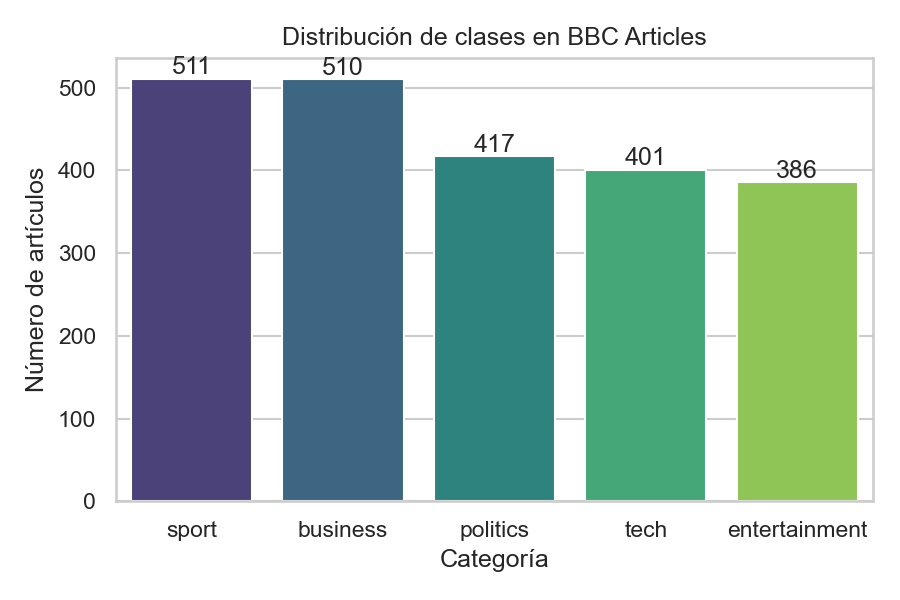
\includegraphics[width=0.85\linewidth]{distribucion_clases.png}
\caption{Distribuci\'on de clases en BBC News. M\'ax/m\'in $\approx$1.32, suficientemente balanceado para reportar m\'etricas \emph{macro} y por clase sin re-balanceo.}
\label{fig:dist}
\end{figure}

\textbf{Arquitectura.} \texttt{BertForSequenceClassification} carga \texttt{bert-base-uncased} (12 capas, 110~M par\'ametros) y a\~nade sobre el \emph{embedding} del token \texttt{[CLS]} un \emph{pooler}, un \texttt{Dropout} y una capa lineal $768\!\to\!5$. La activaci\'on softmax y la \emph{Cross\-Entropy} se aplican internamente en la API, alineando la implementaci\'on con el Micro-proyecto. Justificamos BERT sobre alternativas m\'as ligeras (DistilBERT del laboratorio) por su mayor capacidad y mejor preentrenamiento \cite{bert}, y la variante \emph{uncased} porque el dominio period\'istico no depende de may\'usculas para distinguir clases.

\textbf{Tokenizaci\'on y entrenamiento.} \texttt{padding="max\_length"}, \texttt{truncation=True}, \texttt{max\_length=256}; cubre el \emph{lead} period\'istico --donde se concentra la se\~nal tem\'atica-- a un cuarto del coste de \texttt{max\_length=512}. Fine-tuning end-to-end con \texttt{AdamW} (\emph{weight decay} 0.01, exceptuando \texttt{bias} y \texttt{LayerNorm}), \emph{lr} principal $2\!\times\!10^{-5}$, \emph{linear schedule with warmup} (10\%), \emph{batch size} 16, \emph{gradient clipping} a norma 1.0 y 3 \'epocas (rango 2--5 sugerido). \emph{Seed} fijado en 42; conservamos el \emph{checkpoint} con mejor F1 \emph{macro} de validaci\'on. Para evaluar sensibilidad, replicamos el experimento con \emph{lr}=$5\!\times\!10^{-5}$. M\'etricas reportadas: \emph{accuracy}, \emph{precision}, \emph{recall} y F1 (macro y por clase) sobre \emph{test}, complementadas con la matriz de confusi\'on. Usamos F1 \emph{macro} como criterio principal por ser insensible al desbalance leve.

\section{Resultados}

\textbf{Desempe\~no global.} La configuraci\'on principal alcanza en \emph{test} \textbf{accuracy} = 0.9910 y \textbf{F1 macro} = 0.9909 con \emph{loss} = 0.0394 (Tabla~\ref{tab:resumen}); de los 334 art\'iculos solo 3 se clasifican mal. La variante con \emph{lr}=$5\!\times\!10^{-5}$ alcanza un F1 de validaci\'on m\'aximo m\'as alto (0.994 vs.\ 0.988) y converge antes, pero produce las \emph{mismas} 3 predicciones err\'oneas en \emph{test} -- el dataset est\'a cerca de la saturaci\'on y el margen se manifiesta en confianza, no en aciertos.

\begin{table}[h]
\centering
\caption{Comparaci\'on de configuraciones (BERT-base, 3 \'epocas).}
\label{tab:resumen}
\resizebox{8.5cm}{!}{
\begin{tabular}{lcccc}
\toprule
Config. & Val F1 m\'ax & Test acc. & Test F1 macro & Test loss \\
\midrule
\textbf{lr=$2\!\times\!10^{-5}$} & 0.9878 & \textbf{0.9910} & \textbf{0.9909} & 0.0394 \\
lr=$5\!\times\!10^{-5}$ & 0.9936 & 0.9910 & 0.9909 & 0.0458 \\
\bottomrule
\end{tabular}}
\end{table}

\textbf{Curvas y resultados por clase.} La Fig.~\ref{fig:curvas} muestra que la \emph{loss} de entrenamiento desciende de 0.85 a 0.035 mientras la de validaci\'on se estabiliza en $\sim$0.05; la brecha train/val al final es $<$0.6~p.p.\ en F1, sin sobreajuste pronunciado. Por clase, \emph{entertainment} y \emph{sport} se clasifican perfectamente (F1=1.0) gracias a un l\'exico altamente espec\'ifico y consistente. Las clases m\'as fr\'agiles son \emph{tech} (F1=0.984; \emph{recall}=1.0 pero \emph{precision}=0.968) y \emph{politics} (F1=0.984; \emph{precision}=1.0 pero \emph{recall}=0.968). El patr\'on es asim\'etrico: \emph{tech} \emph{atrae} falsos positivos (al modelo le tienta clasificar como \emph{tech} cuando el l\'exico tecnol\'ogico es saliente) mientras que \emph{politics} \emph{pierde} muestras hacia \emph{business} y \emph{tech}. \emph{Mejor clase}: \emph{entertainment}; \emph{peor clase}: \emph{tech}.

\begin{figure}[h]
\centering

\includegraphics[width=0.95\linewidth]{curvas_entrenamiento.png}
\caption{Curvas de p\'erdida (izq.) y F1 macro (der.) por \'epoca. La validaci\'on supera al entrenamiento en la \'epoca 1 por el efecto regularizador del \texttt{Dropout} en \emph{train}.}
\label{fig:curvas}
\end{figure}

\textbf{Resultados cualitativos.} Aciertos prototipicos con probabilidad softmax $\approx$0.99 (e.g.\ una nota sobre los Oscar etiquetada \emph{entertainment}, $p$=0.9909). Los \emph{tres} errores absolutos del modelo en \emph{test} son tem\'aticamente cre\'ibles y comparten un patr\'on com\'un --la frontera \emph{politics/business/tech}--: (i) ``UK pledges £1bn to vaccine effort'' (real \emph{politics} $\rightarrow$ pred.\ \emph{business}, $p$=0.555); (ii) ``UK firms embracing e-commerce'' (\emph{politics} $\rightarrow$ \emph{tech}, $p$=0.851); (iii) ``Card fraudsters targeting web'' (\emph{business} $\rightarrow$ \emph{tech}, $p$=0.885). En los tres, la etiqueta predicha es una lectura editorial igualmente defendible. Adem\'as, el caso de menor confianza absoluta del \emph{test} ($p$=0.555) coincide con un error, y los siguientes dos casos m\'as dudosos ($p\!\approx\!0.81$--0.82) son aciertos --el softmax act\'ua como un detector calibrado de ambig\"uedad y sugiere que un umbral de rechazo $p\!<\!0.6$ capturar\'ia los fallos genuinos sin descartar muchos aciertos (Fig.~\ref{fig:cm}).

\begin{figure}[h]
\centering
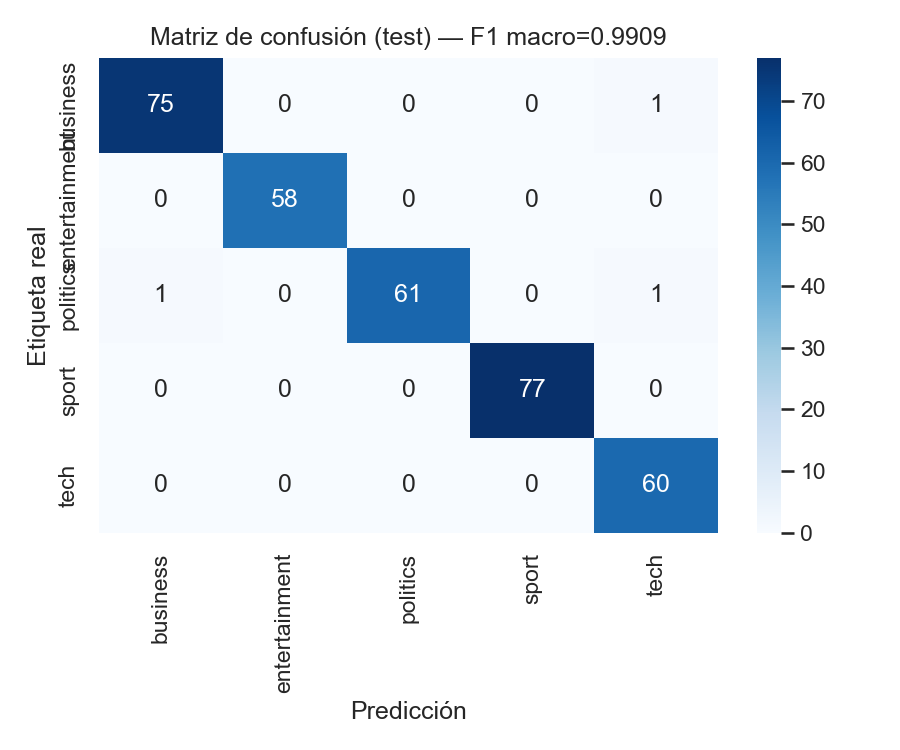
\includegraphics[width=0.78\linewidth]{matriz_confusion.png}
\caption{Matriz de confusi\'on en \emph{test} (BERT-base, lr=$2\!\times\!10^{-5}$): solo 3 errores de 334 muestras.}
\label{fig:cm}
\end{figure}

\section{Discusi\'on}

\textbf{Interpretaci\'on.} El F1 macro de 0.991 confirma que el preentrenamiento bidireccional de BERT \cite{bert} sobre Wikipedia y BookCorpus transfiere de forma efectiva al dominio period\'istico de la BBC: tres \'epocas de fine-tuning sobre 1\,557 muestras bastan para capturar la sem\'antica tem\'atica. Las dos configuraciones (lr=$2\!\times\!10^{-5}$ y $5\!\times\!10^{-5}$) producen las \emph{mismas} 3 predicciones err\'oneas en \emph{test} con \'unicamente diferencias en la calibraci\'on del softmax, lo que indica que el dataset est\'a cerca del techo del benchmark. Los errores residuales no son ruido del modelo sino ambig\"uedad genuina en la frontera \emph{politics/business/tech}, donde la etiqueta canonica de la BBC no es la \'unica lectura razonable.

\textbf{Conexi\'on con la teor\'ia.} Las curvas no muestran sobreajuste cl\'asico (\emph{val\_loss} creciente) en 3 \'epocas y la \emph{val\_loss} a\'un desciende en la \'ultima --2 \'epocas extra exprimir\'ian un margen marginal-- pero el ratio capacidad/datos (110~M par\'ametros vs.\ 1\,557 muestras) hace que un horizonte de m\'as de 5 s\'i deteriorar\'ia la generalizaci\'on; coincide con la recomendaci\'on de \cite{bert} de mantener el fine-tuning corto. El estudio de \emph{lr} ilustra el cl\'asico compromiso sesgo-varianza: $5\!\times\!10^{-5}$ tiene mayor varianza pero llega antes al m\'inimo; $2\!\times\!10^{-5}$ es m\'as conservador. La saturaci\'on en \emph{test} indica que la capacidad del modelo excede la complejidad de la tarea -- escenario propicio para \emph{distillation}. Adicionalmente, el softmax act\'ua como un detector calibrado de ambig\"uedad: el \'unico error con probabilidad $<\!0.6$ \emph{coincide} con el caso de menor confianza absoluta del \emph{test}, sugiriendo que un umbral de rechazo $p\!<\!0.6$ ser\'ia un mecanismo simple de \emph{abstention} en producci\'on.

\textbf{Limitaciones y mejoras.} (i) Dataset peque\~no de un solo medio: el modelo aprende sesgos editoriales brit\'anicos. (ii) Truncar a 256 \emph{tokens} ignora $\sim$50\% del contenido en art\'iculos largos. (iii) Solo se evalu\'o un \emph{seed}; promediar 3--5 dar\'ia intervalos m\'as robustos. (iv) Cinco categor\'ias amplias hacen la tarea relativamente sencilla. Mejoras propuestas: \emph{Hierarchical Transformers} para procesar art\'iculos completos, \emph{distillation} a DistilBERT, y variantes preentrenadas con \emph{span corruption} como T5 \cite{t5} que han mostrado mejoras consistentes en transferencia text-to-text.

\begin{thebibliography}{99}
\bibitem{attention} A. Vaswani \emph{et al.}, ``Attention Is All You Need,'' in \emph{Adv. Neural Inf. Process. Syst. (NeurIPS)}, 2017.
\bibitem{bert} J. Devlin, M.-W. Chang, K. Lee, and K. Toutanova, ``BERT: Pre-training of Deep Bidirectional Transformers for Language Understanding,'' in \emph{Proc. NAACL-HLT}, 2019, pp. 4171--4186.
\bibitem{t5} C. Raffel \emph{et al.}, ``Exploring the Limits of Transfer Learning with a Unified Text-to-Text Transformer,'' \emph{J. Mach. Learn. Res.}, vol. 21, no. 140, pp. 1--67, 2020.
\bibitem{rnn_vs_tx} L. Tunstall, L. von Werra, and T. Wolf, ``Recurrent Neural Networks vs.\ Transformers,'' in \emph{Natural Language Processing with Transformers}, O'Reilly, 2022.
\bibitem{bbcdata} J. Ferretti, ``BBC Articles Dataset,'' Kaggle, 2023. [Online]. Available: \texttt{kaggle.com/datasets/jacopoferretti/bbc-articles-dataset}
\bibitem{hf} T. Wolf \emph{et al.}, ``Transformers: State-of-the-Art Natural Language Processing,'' in \emph{Proc. EMNLP: System Demonstrations}, 2020, pp. 38--45.
\end{thebibliography}

\end{document}
